\section{Right Inverses}

For
\[
    A =
    \begin{bmatrix}
        -1 & 0 & 0 & -1 & 1 \\
        0 & 1 & 1 & 0 & 0 \\
        1 & 0 & 0 & 1 & 0
    \end{bmatrix}
\]
we first solve \(Az=y\). With \(z=[z_1,\ldots,z_5]^\top\), the equations
are
\[
    -z_1-z_4+z_5=y_1,\qquad
    z_2+z_3=y_2,\qquad
    z_1+z_4=y_3.
\]
So \(z_1\), \(z_2\), and \(z_4\) are free, with
\[
    z_3=y_2-z_2,\qquad z_5=y_1+y_3.
\]
Applying this to the standard basis vectors \(y=\{\mathbf{e}_1,\mathbf{e}_2,\mathbf{e}_3\}\), every right inverse has the form
\[
    B =
    \begin{bmatrix}
        a_1 & a_2 & a_3 \\
        b_1 & b_2 & b_3 \\
        -b_1 & 1-b_2 & -b_3 \\
        -a_1 & -a_2 & 1-a_3 \\
        1 & 0 & 1
    \end{bmatrix}
\]
where \(a_i,b_i\in\mathbb{R}\). For any such choice, \(AB=I\).

\textbf{(a)} Yes
\[
    B =
    \begin{bmatrix}
        0 & 0 & 0 \\
        0 & 0 & 0 \\
        0 & 1 & 0 \\
        0 & 0 & 1 \\
        1 & 0 & 1
    \end{bmatrix}.
\]

\begin{figure}[h]
    \centering
    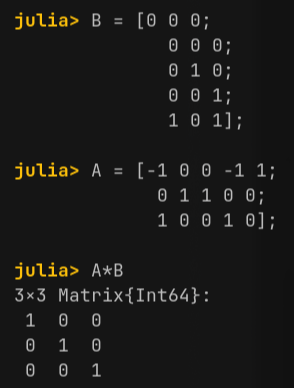
\includegraphics[width=0.3\textwidth]{img/5a.png}
    % \caption{Julia verification for problem 5(a).}
\end{figure}

\textbf{(b)} No. If \(AB=I\) and \(Bx=0\), then
\[
    x = Ix = ABx = A0 = 0.
\]

So \(\operatorname{null}(B)=\{0\}\), which has dimension zero, not one.

\textbf{(c)} No. If the third column of \(B\) were zero, then the third column of
\(AB\) would also be zero. But \(AB=I\), so the third column must be
\(\mathbf{e}_3\neq 0\).

\textbf{(d)} Yes

\[
    B =
    \begin{bmatrix}
        0 & 0 & 0 \\
        0 & 1/2 & 0 \\
        0 & 1/2 & 0 \\
        0 & 0 & 1 \\
        1 & 0 & 1
    \end{bmatrix}.
\]

\begin{figure}[h]
    \centering
    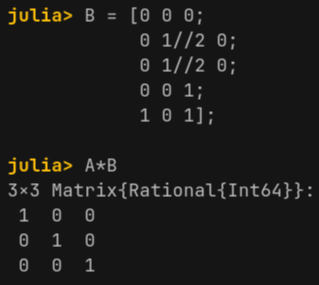
\includegraphics[width=0.3\textwidth]{img/5d.png}
\end{figure}

\textbf{(e)} No. Every right inverse has fifth row \(\begin{bmatrix}1&0&1\end{bmatrix}\), so \(B_{51}=B_{53}=0\), is impossible.

\textbf{(f)} Yes. The matrix from part (a).